%
% METU Institute of Natural and Applied Sciences Thesis example 
%
% Edited and Commented by Utku Erdoğdu 2012
%
% Please read the explanations so that you can customize the document
%
% Files needed by this document:
% metu.cls 
% metu11.def (if you will use 11pt fonts) 
% metu12.def (if you will use 12pt fonts)
% metu10.def (if you will use 10pt fonts)
%
% Possible Options Here:
%
% oneandhalf, double, single : Line spacing used in the thesis. Default and institute preference is
% oneandhalf.
%
% 10pt, 11pt, 12pt : Font size Default is 12pt, which is institute choice. 
% 
% pntr, pntc, pnbt : Page number position. Options are top center, top right or bottom. Default and
% institute preference is page numbers at bottom. When page numbers are at the top bottom margins
% are skewed.
% 
% chaproman, chaparabic : Chapter numbering format. Options are roman numbers and arabic numbers.
% Default is roman, institute prefers arabic
%
% oneside, twoside : Printing style. Default is twoside, which is institute choice. In this style
% chapters begin from odd numbered pages.
%
% threejury, fivejury : For master's degree choose threejury. For doctorate degree choose fivejury.
%
% tr, eng : Document language. This is useful if you want to translate your thesis into
% Turkish. Then you give the option tr and use \ifturkish. . .\else. . .\fi  whenever you want 
% to do something only for Turkish or only for English. Default is eng. 
% IMPORTANT!! : For official institute documents you should not use this option. 
% The Turkish format is only supplied for custom translations.
%
% ceng,aee,arme.. : You can use the abbreviated form of your department here and there is no further need to
% define the department name below. If your department name is not among the below list of defined
% departments, you should use \department and \turkishdepartment macros to define the name of your
% department.
%
% Defined Departments and Abbreviations:
% --------------------------------------
% Computer Engineering : ceng
% Aerospace Engineering : aee
% Archaeometry : arme
% Architecture : arch
% Biochemistry : bch
% Biology : biol
% Biomedical Engineering : bme
% Biotechnology : btec
% Building Science : bs
% Cement Engineering : ceme
% Chemical Engineering : che
% Chemistry : chem
% City and Regional Planning : crp
% City Planning : cp
% Civil Engineering : ce
% Computational Design and Fabrication Technologies in Architecture : arcd
% Computer Education and Instructional Technology : cte
% Design Research for Interaction : iddi
% Earthquake Studies : eqs
% Earth System Science : ess
% Electrical and Electronics Engineering : ee
% Engineering Management : em
% Engineering Sciences : es
% Environmental Engineering : enve
% Food Engineering : fde
% Geodetics - Geographical Information Technologies : ggit
% Geological Engineering : geoe
% Hydrosystems Engineering : he
% Industrial Design : id
% Industrial Engineering : ie
% Mathematics : math
% Mechanical Engineering : mech
% Metallurgical and Materials Engineering : mete
% Micro and Nanotechnology : mnt
% Mining Engineering : mine
% Operational Research : or
% Petroleum and Natural Gas Engineering : pete
% Physics : phys
% Polymer Science and Technology : pst
% Regional Planning : rp
% Restoration : rest
% Secondary Science and Mathematics Education : ssme
% Software Engineering : se
% Statistics : stat
% Structural Mechanics : st
% 
% phd, ms : Degree Received. Ph.D. or M.S. Default is Ph.D..
%
% End of Options

\documentclass[chaparabic,id,phd,12pt,oneandhalf,fivejury]{metu}


\usepackage[table,xcdraw]{xcolor}
\usepackage{csquotes}
\usepackage{appendix}
\usepackage{longtable}
\usepackage{lscape}
\usepackage[pdftex]{hyperref}
\pdfstringdefDisableCommands{\let\uppercase\@firstofone}
\usepackage[all]{hypcap}
\usepackage{todonotes}
\usepackage{graphicx}
\graphicspath{ {./images/} }
\usepackage[figuresright]{rotating}
\usepackage{xy} 
\usepackage{booktabs}
\usepackage{pifont}
\usepackage{color}
\usepackage{listings}
\usepackage{pdfpages}
\usepackage{array}
\usepackage{algorithm}
\usepackage{algorithmic}
\usepackage{float}
\usepackage{caption}
\usepackage{lastpage}
\usepackage{afterpage}
\usepackage{lipsum}
\usepackage{adjustbox}
\usepackage{rotating}
\usepackage{comment}
\usepackage{amsmath,amssymb} % define this before the line numbering.
\usepackage{svg}
\usepackage{color}
\usepackage{enumitem}
\usepackage[normalem]{ulem}
\useunder{\uline}{\ul}{}
\renewcommand{\sectionautorefname}{\S}
\renewcommand{\subsectionautorefname}{\S}
\newcommand{\norm}[1]{\left\lVert#1\right\rVert}
\captionsetup{belowskip=12pt,aboveskip=8pt}
\newcommand{\tab}{\hspace*{2em}}
\DeclareGraphicsExtensions{.pdf,.png,.jpg}
\usepackage{multirow}
\usepackage{amsmath}
\usepackage{siunitx}
\usepackage{textcomp}
\usepackage{subcaption}
\usepackage{enotez}
\usepackage{threeparttable}
\usepackage{layouts}
\usepackage{tikz}
\usepackage{mathtools}

%Uncomment the following line to temporarily show a frame on the page, representing margins. Useful for checking if any figures or tables are overflowing. Make sure to comment it back before production.
%\usepackage[showframe,pass]{geometry}


\DeclarePairedDelimiter\ceil{\lceil}{\rceil}
\DeclarePairedDelimiter\floor{\lfloor}{\rfloor}

%[Turns DOI numbers into links without repeating dx.doi.org each time]
\newcommand{\doi}[1]{doi: \href{http://dx.doi.org/#1}{\nolinkurl{#1}}}
  \newcommand{\EA}[1]{\textcolor{red}{[EA: #1]}}


%%%%%%%%%%%%%%%%%%%%%%%%%%%%%%%%%%%%%%%%%%%%%%%%%%%%%%%%%%%%
%PRELIMINARIES

% 1. Name and Surname
\author{Emre Çağlar}


%%%%%%%%%%%%%%%%%%%%%%%%%%%%%%%%%%%%%%%%%%%%%%%%%%%%%%%%%%%%
% 2. Thesis Title English and Turkish
\title{Exploring Futures with World Building in Design Education: Building and Applying a Theoretical Model Through Action Research}
\turkishtitle{Tasarım Eğitiminde Dünya Kurgulama ile Geleceği Keşfetmek: Eylem Araştırması ile Kuramsal Model Oluşturulması ve Kullanımı}


%%%%%%%%%%%%%%%%%%%%%%%%%%%%%%%%%%%%%%%%%%%%%%%%%%%%%%%%%%%%
% 3. Jury Date
\date{February 2021}


%%%%%%%%%%%%%%%%%%%%%%%%%%%%%%%%%%%%%%%%%%%%%%%%%%%%%%%%%%%%
% 4. Committee 
%
% Use the following abbreviations for people:
% prof : Prof. Dr.
% assocprof : Assoc. Prof. Dr.
% assistprof : Assist. Prof. Dr.
% dr : Dr.
%%%%%%%%%%%%%%%%%%%%%%%%%%%%%%%%%%%%%%%%%%%%%%%%%%%%%%%%%%%%%
% 4A. Director of Institute
\director[prof]{Halil Kalıpçılar}

%%%%%%%%%%%%%%%%%%%%%%%%%%%%%%%%%%%%%%%%%%%%%%%%%%%%%%%%%%%%
% 4B. Head of Department
\headofdept[prof]{Gülay Hasdoğan}
%

%%%%%%%%%%%%%%%%%%%%%%%%%%%%%%%%%%%%%%%%%%%%%%%%%%%%%%%%%%%%
% 4C. Supervisor : English and Turkish
\supervisor[prof]{Gülay Hasdoğan}
% \turkishsupervisor{  } %if you will hard-code the academic title
%
% Affiliation of Supervisor in English and possibly in Turkish
\departmentofsupervisor{Industrial Design, METU}

%\cosupervisor[dr]{Itır Önal Ertuğrul}
%\departmentofcosupervisor{Robotics Institute, Carnegie Mellon University}
%

%%%%%%%%%%%%%%%%%%%%%%%%%%%%%%%%%%%%%%%%%%%%%%%%%%%%%%%%%%%%
% 4D. Committee Members
% First title is the jury chair. Typically, the member with the highest academic title except your supervisor will be the jury chair. Next is your supervisor. The rest of the order is up to you. Ask your supervisor if you are not sure
%
% Professors (1)
% Associate Professors (2)
% Assistant Professors (3)
% Other (4)
% 
% IMPORTANT:  All affiliatons should fit in a single line
% If affiliation line is broken into two lines you should shorten the affiliation by using 
% abbrevations or any other means
%
\committeememberi[prof]{Owain Pedgley}
\affiliationi{Industrial Design, METU}
% Second committee member is always your supervisor
\committeememberii[prof]{Gülay Hasdoğan}
\affiliationii{Industrial Design, METU}

% IMPORTANT: If you are Ph.D. student your co-supervisor can not be in your 
% examination committee.

% \def\@proftitlename{Prof. Dr.}\def\@tproftitlename{Prof. Dr.}
% \def\@assocproftitlename{Assoc. Prof. Dr.}\def\@tassocproftitlename{Doç. Dr.}
% \def\@assistproftitlename{Assist. Prof. Dr.}\def\@tassistproftitlename{Yrd. Doç. Dr.}
% \def\@drtitlename{Dr.}\def\@tdrtitlename{Dr.}

\committeememberiii[assistprof]{Ali Berkman}
\affiliationiii{Industrial Design, TOBB ETU}
% Fourth committee member
\committeememberiv[assistprof]{Gökhan Mura}
\affiliationiv{Visual Communication Design, Izmir University of Economics}
% Fifth committee member
\committeememberv[assistprof]{Senem Turhan}
\affiliationv{Industrial Design, METU}
%%%%%%%%%%%%%%%%%%%%%%%%%%%%%%%%%%%%%%%%%%%%%%%%%%%%%%%%%%%%%

%%%%%%%%%%%%%%%%%%%%%%%%%%%%%%%%%%%%%%%%%%%%%%%%%%%%%%%%%%%%
% 5. Keywords : English & Turkish, Comma seperated
\keywords{design fiction, design education, world building, design for future, action research}
\anahtarklm{kurgusal tasarım, tasarım eğitimi, dünya kurgulama, gelecek için tasarım, eylem araştırması}
%%%%%%%%%%%%%%%%%%%%%%%%%%%%%%%%%%%%%%%%%%%%%%%%%%%%%%%%%%%%


%%%%%%%%%%%%%%%%%%%%%%%%%%%%%%%%%%%%%%%%%%%%%%%%%%%%%%%%%%%%%
% 6A. Abstract in English
%
\abstract{
Design students are often engaged with future contexts, as design education encourages them to explore different contexts and understand the implications of their activities. These explorations are done in what is called a fuzzy front-end in design, which stands for the chaotic but fruitful early phase of a design process. There are different apporaches used by design students to conduct research and increase immersion into the context in this phase. Approaches such as design scenarios, make use of fictional information in addition to factual, in order to increase immersion into context and help design students generate inferential insights. This creates both epistemological and practical challenges in terms of how to define and utilize fiction within the early phases of design. This study draws from the existing literature to utilize world building in this phase. Through action research, three workshops were conducted with design students to generate a theoretical model for presenting how world building is utilized in design education, contributing to the design literature. Furthermore, the toolset devised for use in these workshops is iterated throughout the study based on the insights from the theoretical model, and is presented as a practical contribution to the design education literature. Based on the results, this study presents a case for how world building in design education is carried out in waves of speculation for creating textual reference worlds, and assessment for comparing these speculations with actuality through pragmatic concerns.
}
%%%%%%%%%%%%%%%%%%%%%%%%%%%%%%%%%%%%%%%%%%%%%%%%%%%%%%%%%%%%%


%%%%%%%%%%%%%%%%%%%%%%%%%%%%%%%%%%%%%%%%%%%%%%%%%%%%%%%%%%%%
% 6B. Turkish Abstract
%
\oz{
Tasarım eğitimi, öğrencilerin farklı bağlamları keşfetmesi ve üretimlerinin bu bağlamları nasıl etkileyebileceğini düşünebilmeleri için onları sıklıkla gelecek bağlamları ile ilgili çalışmaya itmektedir. Bu keşifler tasarımın belirsiz önyüzü de denilen, kaotik fakat üretken bir erken tasarım sürecinde gerçekleşmektedirler. Bu süreçte tasarım öğrencileri pek çok farklı yöntemden faydalanarak araştırma yapar ve önceden tanımadıkları bağlamların içine girmeyi hedeflerler. Bu yöntemlerden biri olan tasarım senaryoları, gerçek bilgilerden olduğu kadar kurgusal bilgilerden de faydalanır. Bu sayede öğrenciler bağlamların daha çok içine girerek dolaylı çıkarımlar yapabilirler. Bu durum, kurgunun tasarımdaki tanımı ve yeri ile ilgili epistemolojik ve pratik sorunları beraberinde getirir. Bu tez, mevcut literatürden faydalanarak söz konusu erken aşamayı bir dünya kurgulama yöntemi olarak tanımlıyor. Tez kapsamında eylem araştırması ile üç çalıştay gerçekleştirilmiş ve sonuç olarak ortaya tasarım eğitiminde dünya kurgulamanın nasıl kullanıldığına dair bir teorik model çıkartılarak tasarım literatürüne katkı sağlanmıştır. Bununla birlikte, çalıştaylarda kullanılan araç seti, çalışma boyunca geliştirilmiş ve son hali ile tasarım eğitimi literatürüne katkı olarak sunulmuştur. Tezin sonucunda tasarım eğitiminde dünya kurgulamanın, önce metinsel referans dünyalarını yaratan spekülasyonlar, sonra da bunları asli dünyadaki pragmatik endişelerle karşılayan değerlendirmeler arasındaki dalgalanmalar olarak tasviri öne sürülmüştür. 
} 

%%%%%%%%%%%%%%%%%%%%%%%%%%%%%%%%%%%%%%%%%%%%%%%%%%%%%%%%%%%%
%7. Dedication
\dedication{Dedication}


%%%%%%%%%%%%%%%%%%%%%%%%%%%%%%%%%%%%%%%%%%%%%%%%%%%%%%%%%%%%
%8. Acknowledgments  
\acknowledgments{
Acknowledgements
}

%
% End of Personal and Introductory Information
%%%%%%%%%%%%%%%%%%%%%%%%%%%%%%%%%%%%%%%%%%%%%%%%%%%%%%%%%%%%

%%%%%%%%%%%%%%%%%%%%%%%%%%%%%%%%%%%%%%%%%%%%%%%%%%%%%%%%%%%%
%REFERENCES
%Add your references to this bib file, included with this template. Connect it to your reference manager, such as Zotero, so that it auto-exports your references to this file at every change. This way, all references in your reference manager will be available to cite in this template.
\addbibresource{bibliography.bib}
%%%%%%%%%%%%%%%%%%%%%%%%%%%%%%%%%%%%%%%%%%%%%%%%%%%%%%%%%%%%

%%%%%%%%%%%%%%%%%%%%%%%%%%%%%%%%%%%%%%%%%%%%%%%%%%%%%%%%%%%%
%SUPPORT FOR REFERENCING MOVIES AND TV-SHOWS
%This enables referencing movies and TV shows. Add movies or TV-shows to the separate films.bib file. See the file for examples.

\addbibresource{films.bib}

\DeclareLabelname[movie]{
	\field{director}
	\field{producer}
}
\DeclareFieldFormat[movie]{entrysubtype}{\mkbibbrackets{#1}}
%%%%%%%%%%%%%%%%%%%%%%%%%%%%%%%%%%%%%%%%%%%%%%%%%%%%%%%%%%%%




%USEFUL TOOLS

%%%%%%%%%%%%%%%%%%%%%%%%%%%%%%%%%%%%%%%%%%%%%%%%%%%%%%%%%%%
% A. Section referencing within text:

% New reference command for section references with full section number and heading. E.g. for "Section 5.2 Design", write \fullref{sec:ws1-design} in which the argument is your label for the linked section. \literef{sec:ws1-design} produces "5.1, p.XX". You can customize your own custom in-text referencing system here.
\newcommand*{\fullref}[1]{\hyperref[{#1}]{\ref*{#1} \nameref*{#1}}}
\newcommand*{\literef}[1]{\hyperref[{#1}]{\ref*{#1}, p.\pageref*{#1}}}
%%%%%%%%%%%%%%%%%%%%%%%%%%%%%%%%%%%%%%%%%%%%%%%%%%%%%%%%%%%%


%%%%%%%%%%%%%%%%%%%%%%%%%%%%%%%%%%%%%%%%%%%%%%%%%%%%%%%%%%%%
% B. Original quotes section in the Appendix
%All endnotes specified in your chapters, using \endnote{...} command, will be put in a seperate Appendix with the title specified below. This way you can put the the original language version of any quotes you want. An example is given in the sample chapters. Remove the %!TEX root =  ../thesis.tex
% Appendix
% \chapter{Original Quotes}
\label{chp:Original Quotes}
\printendnotes[custom] line from the chapters list below if not using.

\DeclareInstance{enotez-list}{custom}{paragraph} {
	notes-sep = \baselineskip,
	format = \normalfont,
	number = \normalfont{[#1]}
}

\setenotez{
	backref=true,
	list-name=,
	list-heading=\chapter{Original Quotes},
	list-style=plain,
	split=chapter,
	split-title=Quotes from Chapter <ref>,
}
%%%%%%%%%%%%%%%%%%%%%%%%%%%%%%%%%%%%%%%%%%%%%%%%%%%%%%%%%%%%

%%%%%%%%%%%%%%%%%%%%%%%%%%%%%%%%%%%%%%%%%%%%%%%%%%%%%%%%%%%%
% C. New Table Columns
% Use L, C, or R in the tabular environment for vertically centered cells with left, center or right aligned text.
\newcolumntype{L}[1]{>{\raggedright\let\newline\\\arraybackslash\hspace{0pt}}m{#1}}
\newcolumntype{C}[1]{>{\centering\let\newline\\\arraybackslash\hspace{0pt}}m{#1}}
\newcolumntype{R}[1]{>{\raggedleft\let\newline\\\arraybackslash\hspace{0pt}}m{#1}}
%%%%%%%%%%%%%%%%%%%%%%%%%%%%%%%%%%%%%%%%%%%%%%%%%%%%%%%%%%%%

\begin{document}
% Preliminaries
\begin{preliminaries}
% If you are willing to use any custom stuff before Chapters, put it here
% Such as List of Abbreviations
% Check the abbreviations.tex for a template list of abbreviations

\begin{theglossary}{LONGESTABBRV}
\item[FFED] Fuzzy Front-End of Design
\item[SCD] Speculative and Critical Design
\item[HCI] Human-Computer Interaction
\end{theglossary}

% End of Preliminaries
\end{preliminaries}
%   
% 
%
\setlength{\parindent}{0em}
\setlength{\parskip}{10pt}

%%%%%%%%%%%%%%%%%%%%%%%%%%%%%%%%%%%%%%%%%%%%%%%%%%%%%%%%%%%%
%CHAPTERS
% You can add as many chapters
%!TEX root =  ../thesis.tex
% CHAPTER 1
\chapter{Introduction}
\label{chp:b1}

	There is an increasing interest in the early stages of design, the so called fuzzy front-end in design (FFED), which focuses on defining better questions before designers attempt to answer them \cite{aaltonenHowWeMake2005}.
	

	\begin{figure}[h!]
			\centering
			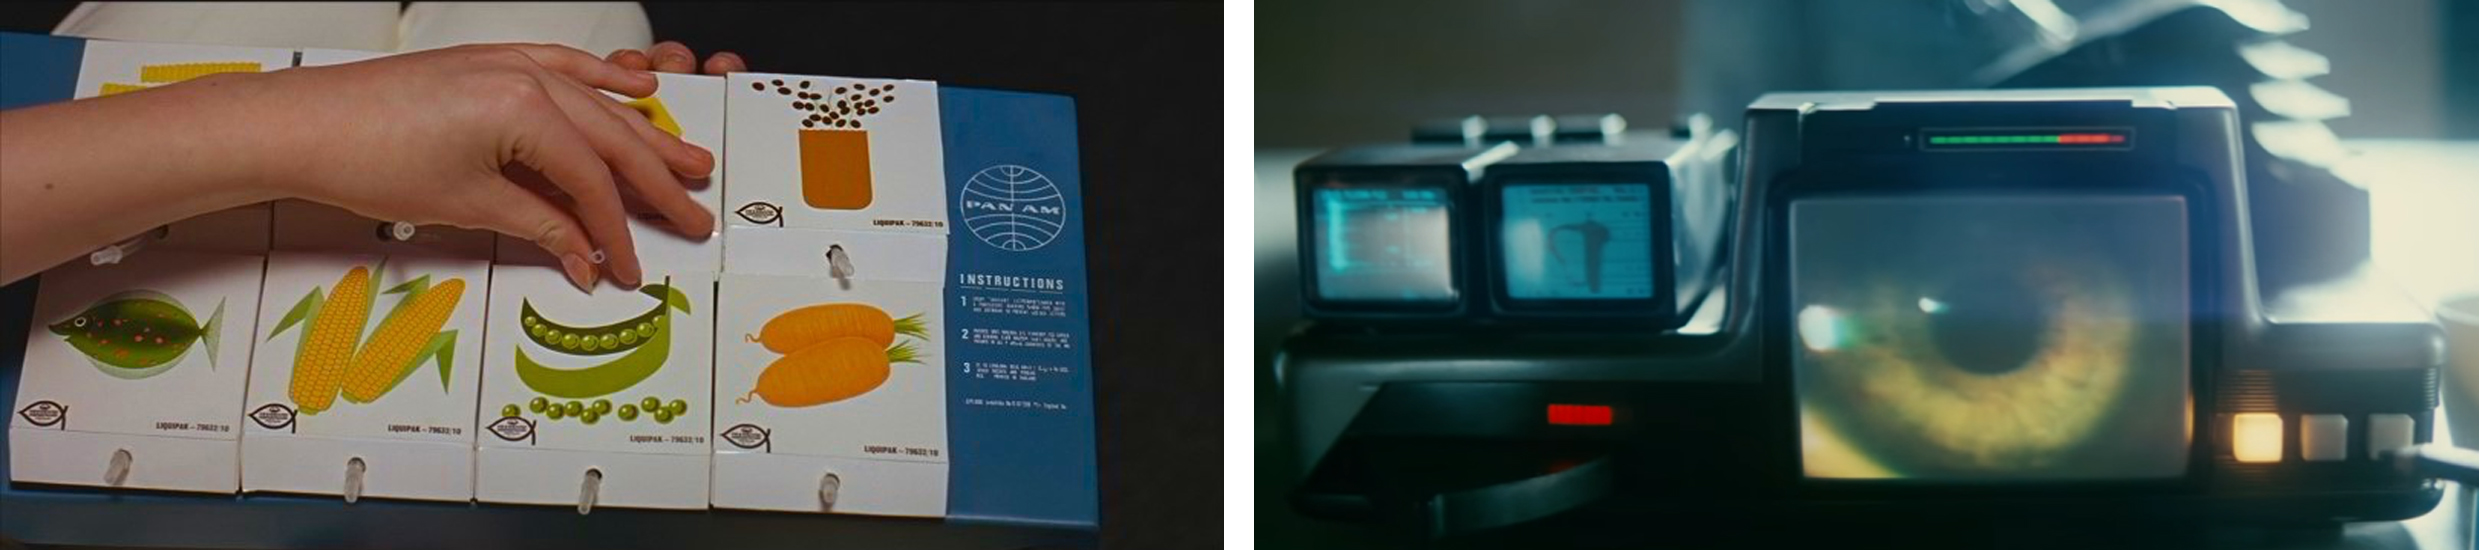
\includegraphics[width=.8\textwidth]{figures/2001-Bladerunner.jpg}
			\caption{Screencaps from a movie \cite{bladeRunner}.}
			\label{fig:movies}
	\end{figure}

	\begin{comment}
		TODO
		Buraya bir bağlantı lazım. Önceki paragrafta lafı design studentlara getirebilirsin.
	\end{comment}

	
	\section{Research Aim}
	

\section{Research Questions and Approach}
\label{Research Questions}
	My aim is to explore world building in design education, by understanding and supporting it in the early phases of design. My main research questions are as follows: 

	\begin{enumerate}
	\item How can a theoretical model describe and represent the world building process of design students when working with future contexts?
	\item What are the properties of a toolset for openly enabling world building to be used by design students when working with future contexts?
	\end{enumerate}


\section{Contributions to Literature}

	There will be two main contributions to the existing body of knowledge in design education. First, the answer to my first research question will provide a theoretical model of world building in design education. This model will be generated by layering four research outputs: (1) an interpretive literature review for transporting concepts of world building from media studies to design, (2) elements and their properties of world building, (3) processes of world building and (4) pragmatic concerns of world building. These layers will be weaved together to present a wholistic model of world building in design education, contributing to existing body of knowledge within design education literature.
	

\section{Structure of the Thesis}
	The overall structure of this dissertation is built on four components: literature review, methodological framework, workshops and conclusions. The literature review consists of Chapter~\ref{chp:b2} (p.~\pageref{chp:b2}), and Chapter~\ref{chp:b3} (p.~\pageref{chp:b3}). These chapters will present my theoretical background. 

%!TEX root =  ../thesis.tex
% CHAPTER 2
\chapter{Literature Review}
\label{chp:b2}

	In this chapter, I will explore the existing approaches used by designers to make sense of unfamiliar contexts \cite{aaltonenHowWeMake2005}.

	\begin{figure}[h!]
	\centering
	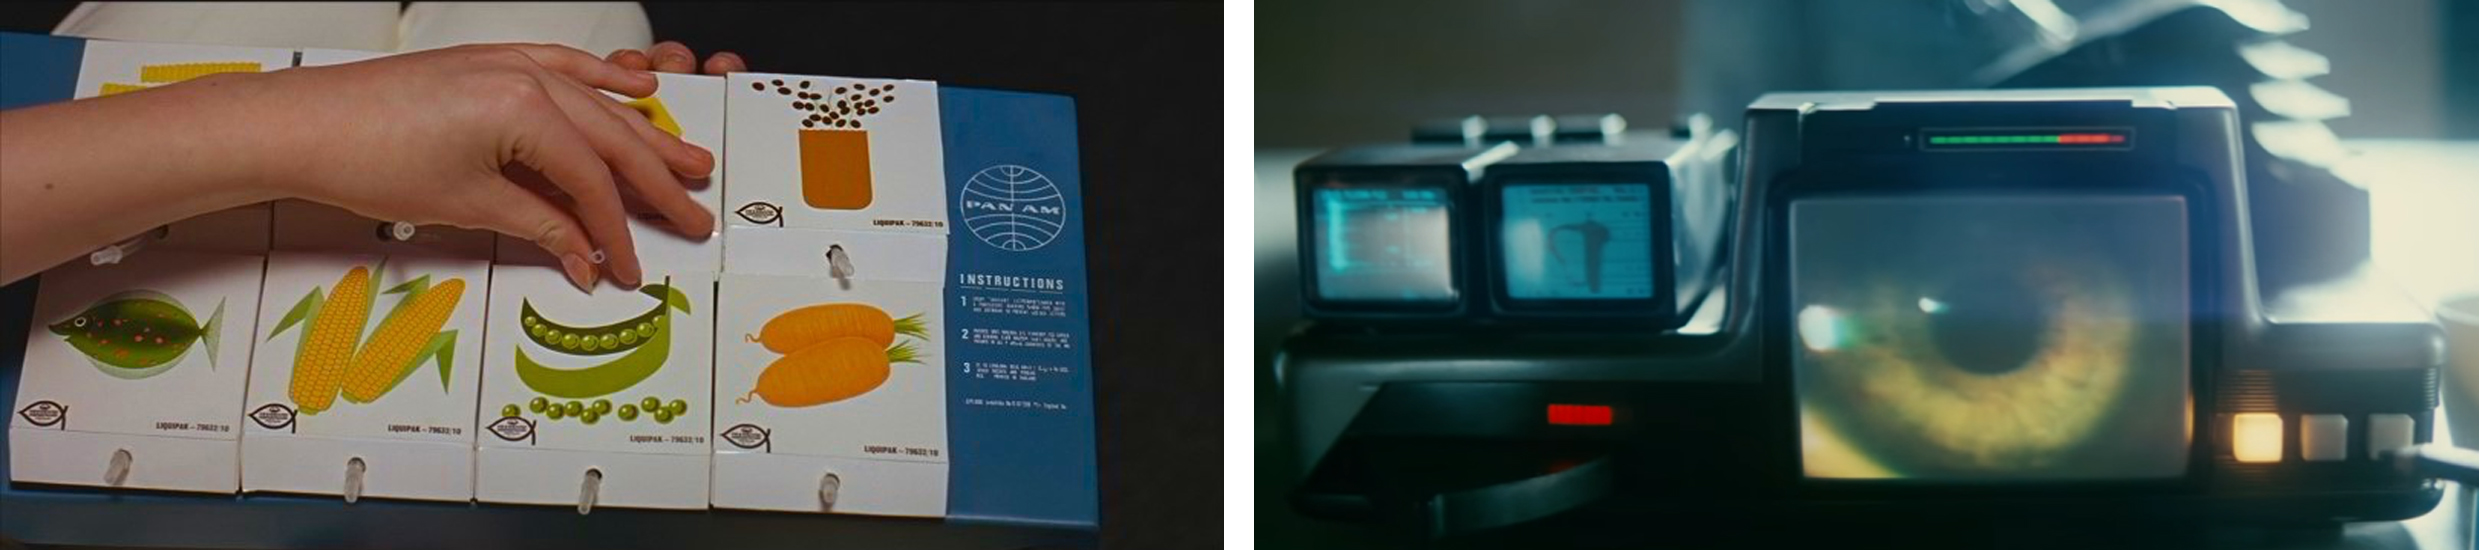
\includegraphics[width=.99\textwidth]{figures/2001-Bladerunner}
	\caption{FFED in the design process.}
	\label{fig:FFED}
	\end{figure}

\section{Heading 1}
Design research is often theorized under three phases: exploratory, generative, and evaluative research.

	\subsection{Subheading}
	\label{subsec:subheading}
	
	\subsubsection{Subsubheading}
	\label{subsubsec:subsubheading}
	Below is a quote I translated from the original Turkish. The original Turkish text is automatically inserted in the Appendix.
	
	\begin{displayquote}
		"English translation from the original quote."\endnote{Orjinal Türkçe metin.}
	\end{displayquote}
	
	Design research is often theorized under three phases: exploratory, generative, and evaluative research \cite{aaltonenHowWeMake2005}. 
%!TEX root =  ../thesis.tex
% CHAPTER 3
\chapter{Methodology}
\label{chp:b3}

In this chapter, I will explore the existing approaches used by designers to make sense of unfamiliar contexts \cite{aaltonenHowWeMake2005}.

\begin{figure}[h!]
	\centering
	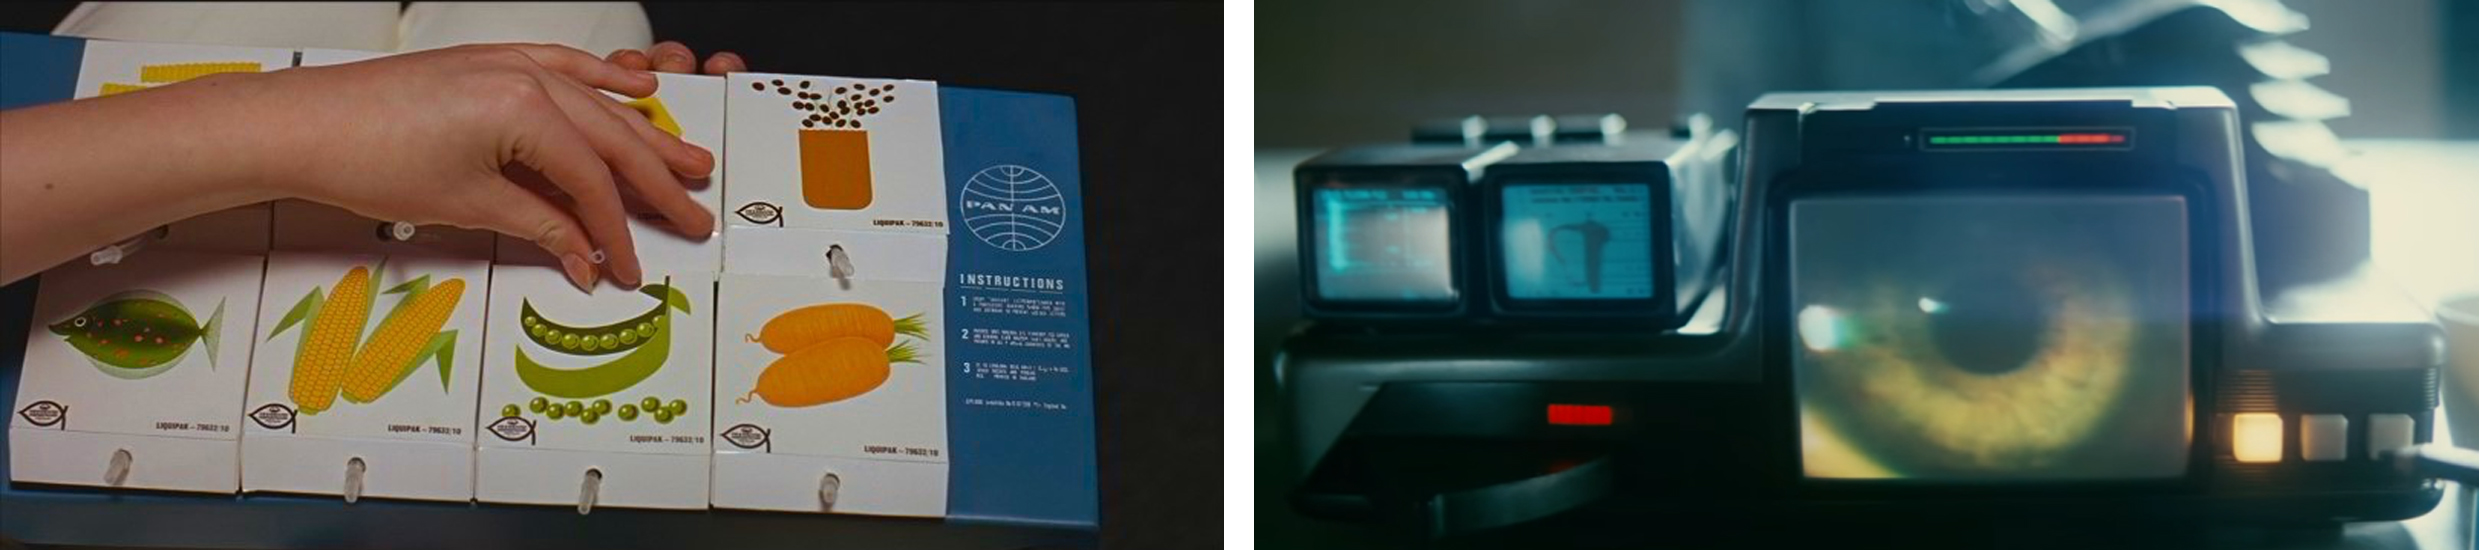
\includegraphics[width=.99\textwidth]{figures/2001-Bladerunner}
	\caption{FFED in the design process.}
	\label{fig:FFED-2}
\end{figure}

\section{Heading 1}
Design research is often theorized under three phases: exploratory, generative, and evaluative research.

\subsection{Subheading}
\label{subsec:subheading-2}

\subsubsection{Subsubheading}
\label{subsubsec:subsubheading-2}

Below is a quote I translated from the original Turkish. The original Turkish text is automatically inserted in the Appendix.

\begin{displayquote}
	"English translation from the original quote."\endnote{Orjinal Türkçe metin.}
\end{displayquote}

Design research is often theorized under three phases: exploratory, generative, and evaluative research \cite{aaltonenHowWeMake2005}. 
%%%%%%%%%%%%%%%%%%%%%%%%%%%%%%%%%%%%%%%%%%%%%%%%%%%%%%%%%%%%

%%%%%%%%%%%%%%%%%%%%%%%%%%%%%%%%%%%%%%%%%%%%%%%%%%%%%%%%%%%%
%REFERENCES
\chapter*{\uppercase{References}}
\addcontentsline{toc}{leads}{\protect\numberline {}\uppercase{REFERENCES}}
\printbibliography[heading=none]
%%%%%%%%%%%%%%%%%%%%%%%%%%%%%%%%%%%%%%%%%%%%%%%%%%%%%%%%%%%%

%%%%%%%%%%%%%%%%%%%%%%%%%%%%%%%%%%%%%%%%%%%%%%%%%%%%%%%%%%%%
%APPENDICES
% If you have more that one appendix, then use \appendices, otherwise use 
% \appendix
\appendices

\addcontentsline{toc}{leads}{\protect\numberline {}\uppercase{APPENDICES}}
% comment out the following line if not using the original quotes function.
%!TEX root =  ../thesis.tex
% Appendix
% \chapter{Original Quotes}
\label{chp:Original Quotes}
\printendnotes[custom]

% Appendices go below. Add as many appendices as you need.
%!TEX root =  ../thesis.tex
% Appendix
\chapter{Sample Appendix}
\label{chp:LabelForAppendix}

A sample Appendix file with sections
\section{Section 1}
Lorem ipsum dolor sit amet, consectetur adipiscing elit. Quisque vel maximus dolor. Nunc ex ex, eleifend vel lacus a, lobortis iaculis turpis. Phasellus eget nibh facilisis urna interdum tincidunt. Donec finibus leo vel mi eleifend, ut suscipit augue sodales. Etiam eu faucibus nulla. Cras sed vulputate erat, ac placerat eros. In hac habitasse platea dictumst. Quisque tincidunt tortor eu nisl pretium aliquet. Praesent elementum est risus, ut faucibus quam efficitur et. Suspendisse varius dui quis ipsum commodo convallis. Donec congue, felis ut tempus vestibulum, nulla nisi euismod orci, ut iaculis dolor turpis id felis. Sed semper pulvinar ipsum, a ultricies enim ultrices nec. Maecenas a urna non dolor gravida tincidunt.

\section{Section 2}
Lorem ipsum dolor sit amet, consectetur adipiscing elit. Quisque vel maximus dolor. Nunc ex ex, eleifend vel lacus a, lobortis iaculis turpis. Phasellus eget nibh facilisis urna interdum tincidunt. Donec finibus leo vel mi eleifend, ut suscipit augue sodales. Etiam eu faucibus nulla. Cras sed vulputate erat, ac placerat eros. In hac habitasse platea dictumst. Quisque tincidunt tortor eu nisl pretium aliquet. Praesent elementum est risus, ut faucibus quam efficitur et. Suspendisse varius dui quis ipsum commodo convallis. Donec congue, felis ut tempus vestibulum, nulla nisi euismod orci, ut iaculis dolor turpis id felis. Sed semper pulvinar ipsum, a ultricies enim ultrices nec. Maecenas a urna non dolor gravida tincidunt.



% Edit the vita.tex file for your CV.
\curriculumvitae
\label{chp:vita}

\section*{\uppercase{Personal Information}}

\textbf{Surname, Name: } Surname, Name\\
\textbf{Nationality:} Turkish (TC) \\
\textbf{Date and Place of Birth:} Birthday, Birthplace\\
\textbf{Marital Status:} Marital Status \\
\textbf{Phone:} Phone Number \\
\textbf{Fax:} Fax Number \\

\section*{\uppercase{Education}}

\begin{tabular}{lll}
	\textbf{Degree} & \textbf{Institution} & \textbf{Year of Graduation} \\
	M.S. & M.S. Institute & M.S. Year \\
	B.S. & B.S. Institute & B.S. Year \\
	High School & High School Name & High School Graduating Year
\end{tabular}

\section*{\uppercase{Professional Experience}}

\begin{tabular}{lll}
	\textbf{Year} & \textbf{Place} & \textbf{Enrollment} \\
	Duration 1 & Institute/Company 1 & Role/Position/Experience 1 \\
	Duration 2 & Institute/Company 2 & Role/Position/Experience 2 
\end{tabular}

\section*{\uppercase{Publications}}
\subsection*{International Conference Publications}
Your publications goes here. Do not try to use Bibtex, since Bibtex builds a single bibliography
database for the document.

\end{document}
